\chapter{MPEG-2 Codec Implementation}
\label{chapter:decoder}

This chapter describes the MPEG-2 decoder and encoder 
implementations written in StreamIt. 
Sections~\ref{decoder_in_streamit} through~\ref{encoder:estimation} explain 
the actual code base and program structure. 
Section~\ref{section:first_decoder_impl} describes the 
specific functionality in the StreamIt implementations
and highlights implementation statistics pertinent to 
the discussion of programmability and parallelism.

\section{Decoder Structure}
\label{decoder_in_streamit}

\begin{figure}[h]
  \begin{center}
    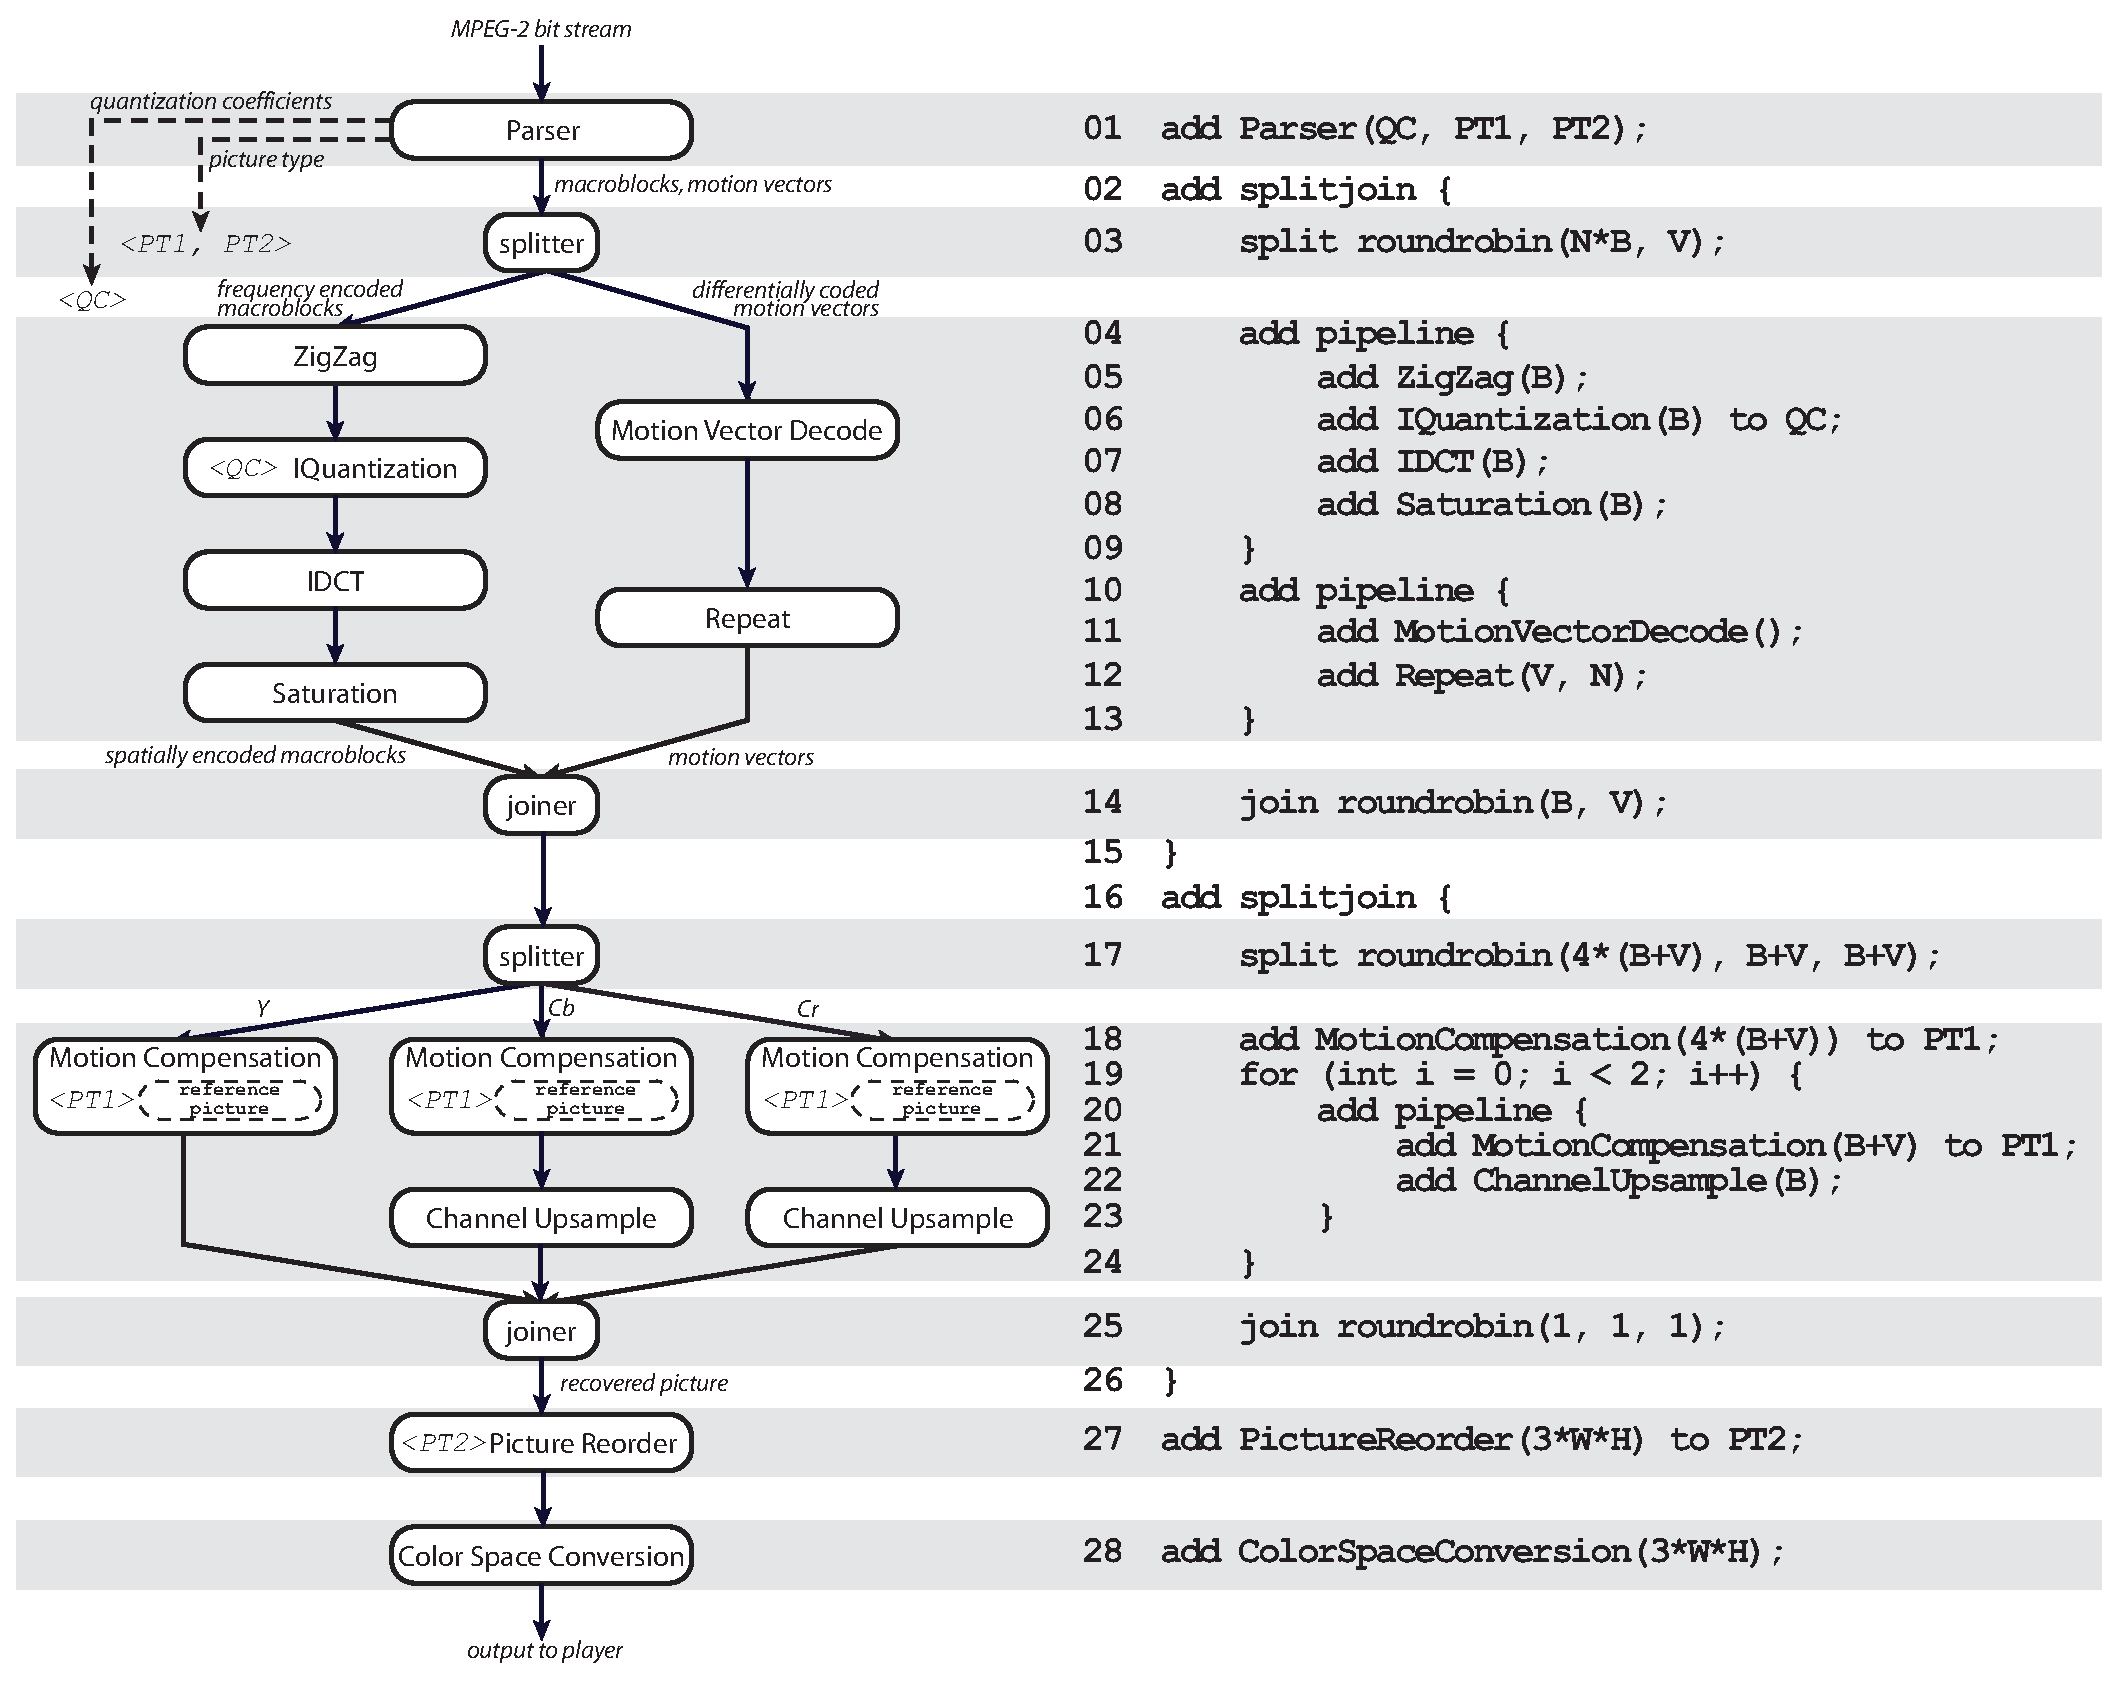
\includegraphics[scale=0.44, angle=0]{./decoder_with_code.eps}
    \caption{MPEG-2 decoder block diagram with associated StreamIt code.}
    \label{fig:dec-with-code}
  \end{center}
\end{figure}

Figure~\ref{fig:dec-with-code} shows the MPEG-2 decoder pipeline, 
correlated with the StreamIt code. A few simplifications have been made 
to the code and the figure for purposes of explanation\footnote{The code 
and figures throughout this paper are meant to highlight important implementation 
details. Figures showing every detail of the MPEG decoder and encoder 
implementations are available on the StreamIt MPEG-2
website~\cite{mpeg-streamit-website} and are not reproduced in an appendix because 
the high level of detail demands an extreme resolution that would be 
unreadable on regular paper sizes.}. 
The decoder accepts a compressed bit stream as input and produces
a decoded video stream as output. The parser (line 1) performs 
variable length decoding (VLD) and interprets the bitstream. 
Because it interprets the bitstream, it dictates decoding parameters 
which are propagated to the appropriate downstream filters using teleport 
messaging. The parser outputs macroblocks sequentially, first emitting the 
blocks contained within a macroblock and then the differentially coded 
motion vectors associated with the macroblock. 

The parser output is segregated into two homogeneous streams by a 
roundrobin splitter (line 3). The first stream contains blocks, 
which are spatially decoded by the block decoder (lines 4-9). The 
second stream is decoded to produce absolute motion vectors (lines 10-13). 
The two streams are merged with a roundrobin joiner (line 14), which 
alternates between a block from the left stream, and a set of motion 
vectors from the right stream.

The next stage of the decoding pipeline performs the motion 
compensation (lines 16-26) to recover predictively coded macroblocks. 
Whereas the first half of the pipeline made a split between block data 
and motion data, the second half of the pipeline splits data 
according to color channel. The splitter (line 17) first segregates 
the luminance data into the left stream, and the two sets of 
chrominance data into the middle and right streams. The exact 
amount of data sent each way in this splitter is dependent on the 
chroma format of the video. The motion compensation filters each 
take in block data and motion vector data to find a corresponding 
macroblock in a previously decoded reference picture. The reference 
macroblock is added to the current macroblock to recover the original 
picture data. Reference pictures are stored within the decoder for future 
use. 

The two chrominance channels each require upsampling so that every pixel 
in a video has a value. Finally, the color channels are merged by a 
joiner (line 25) which merges one item at a time from each stream so 
that each pixel occurs sequentially.

The final two stages of decoding are picture reordering and color 
channel conversion. Picture reordering (line 27) ensures that the data 
is emitted in temporal order, and the color space conversion (line 28) 
ensures that the data is in the correct output format. 

\section{Encoder Structure}

\begin{figure}[h]
  \begin{center}
    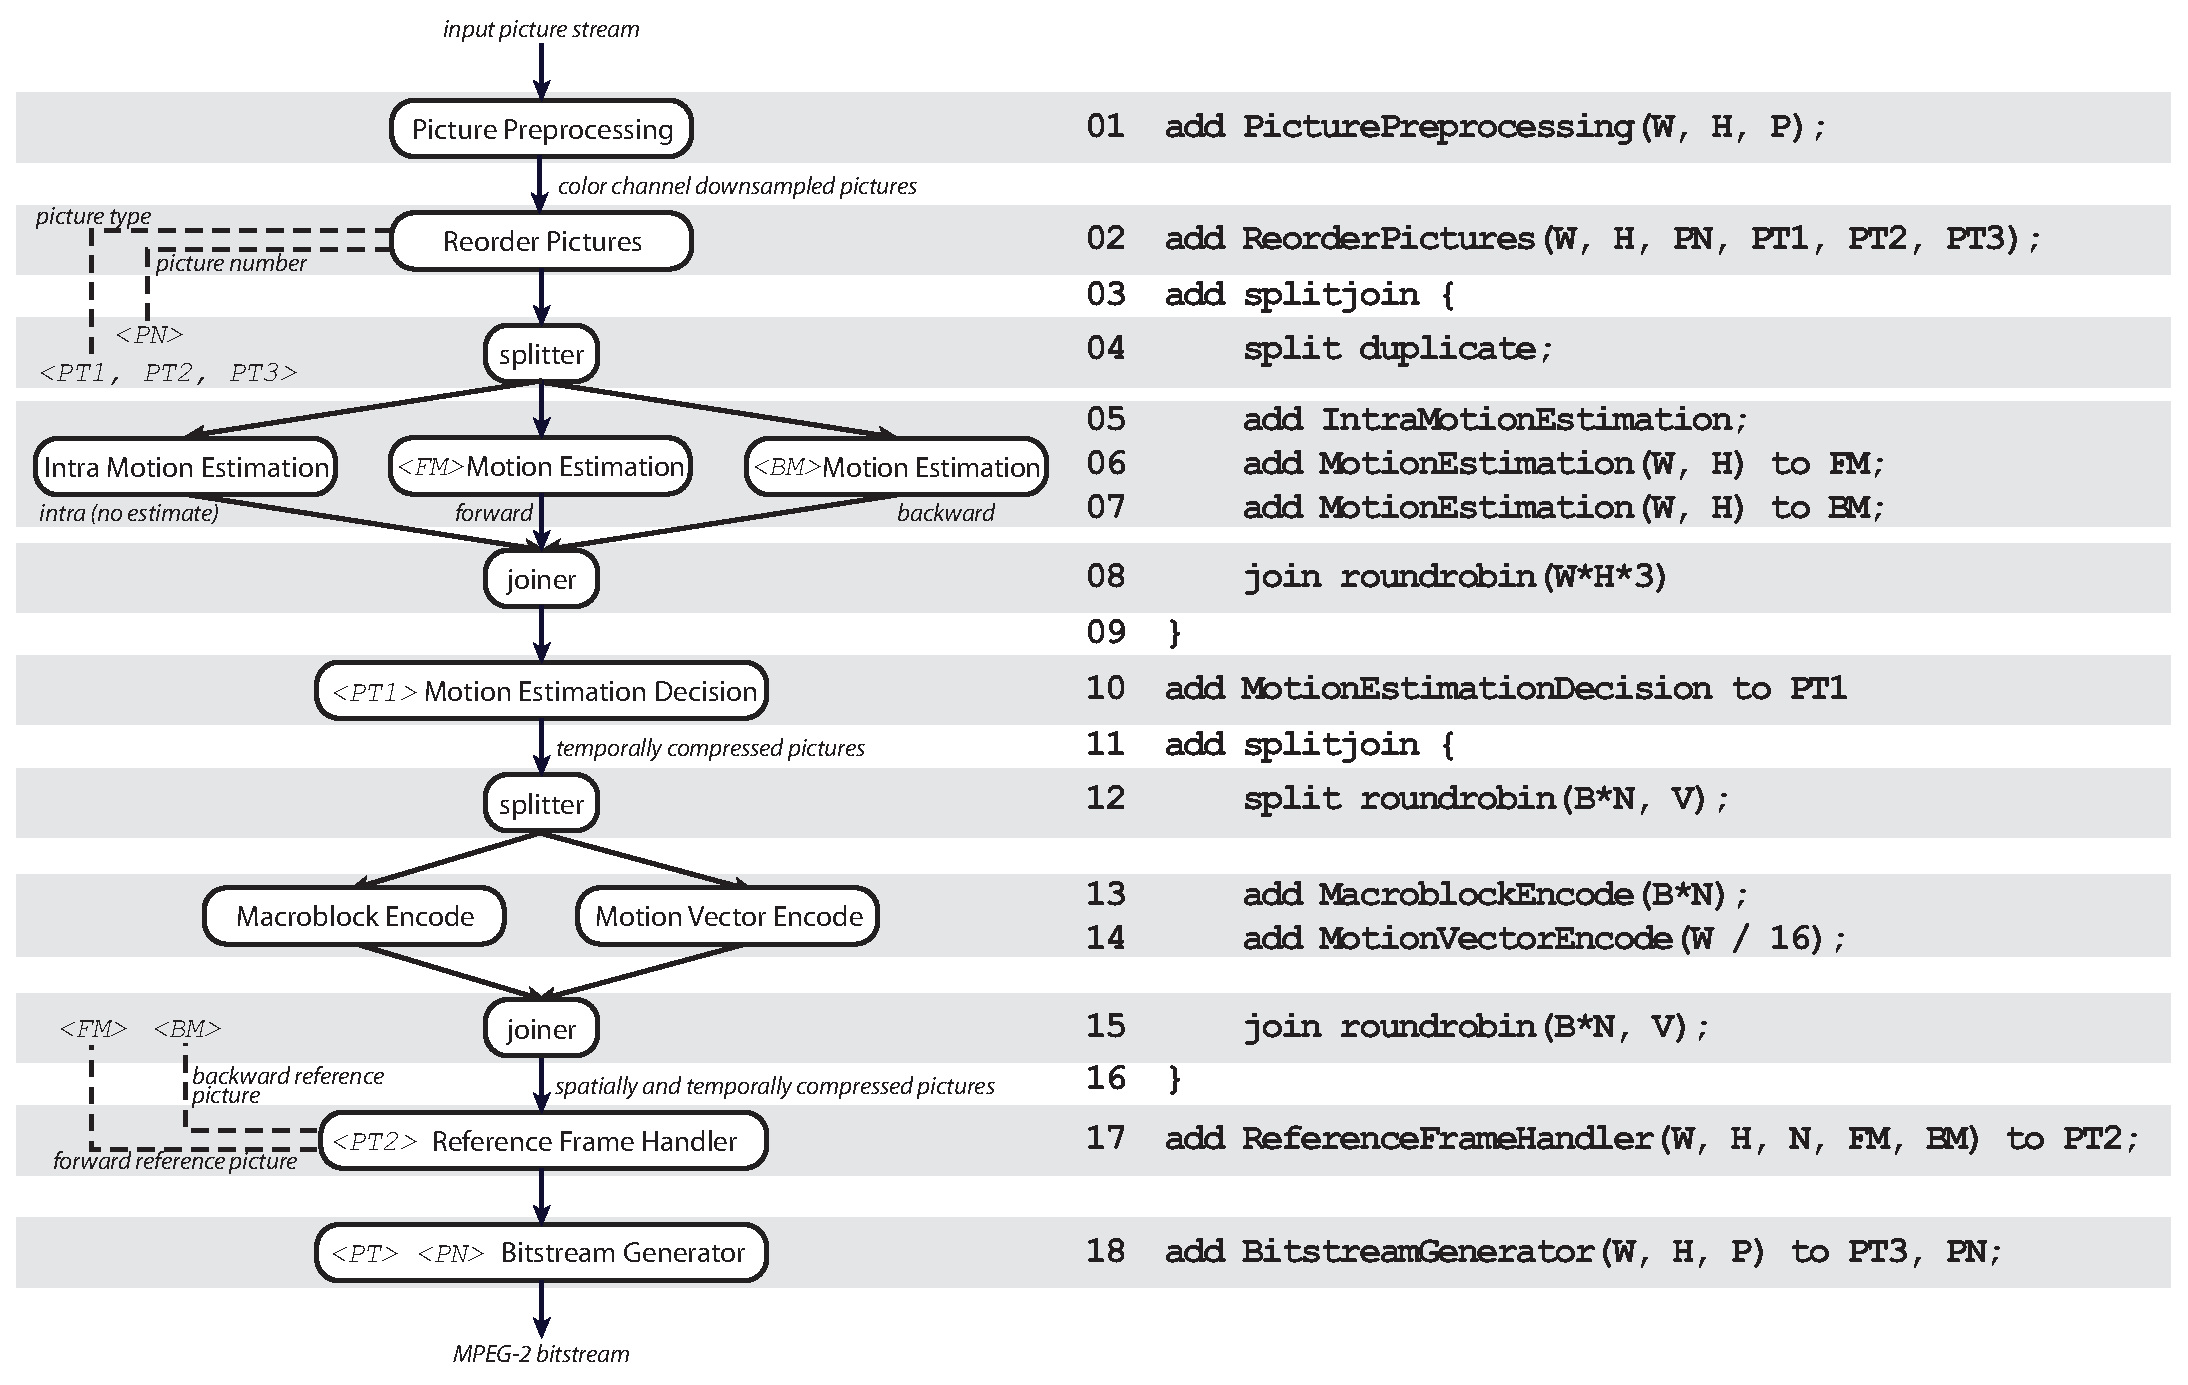
\includegraphics[scale=0.4, angle=0]{./encoder_with_code.eps}
    \caption{MPEG-2 encoder block diagram with associated StreamIt code.}
    \label{fig:encoder-with-code}
  \end{center}
\end{figure}

Figure~\ref{fig:encoder-with-code} shows the MPEG-2 encoder 
pipeline, correlated with the StreamIt code. Because the MPEG-2 
encoder is a larger application and many subcomponents have been 
explained in the decoder, it is presented at a higher level of abstraction. 

The encoder accepts a series of pictures as input and produces a coded 
bit stream as output. A picture preprocessor (line 1) downsamples the color 
channels and assigns an I, P, or B picture type to each 
picture. The output is reordered (line 2) so that all reference 
pictures precede pictures that use them as references. The component 
responsible for reordering also sends this information via message to 
downstream filters which have behavior dependent on the picture 
type. The output of the picture reorder filter is a sequence of 
pictures, ordered by macroblock and then block.

The reordered picture output is then motion estimated (lines 3-10) 
to determine the relative motion of each picture with respect to 
reference pictures. This component receives upstream messages which 
tell it what reference frames the decoder will have available, 
and what they look like.
Because the motion estimation has some particularly interesting 
implementation issues, a more detailed explanation of its behavior 
follows in Section~\ref{encoder:estimation}.

The motion estimation outputs a series of interleaved blocks and 
motion vectors. A splitter (line 12) separates these blocks and 
motion vectors. The blocks are spatially coded (line 13) and the 
motion vectors differentially coded (line 14) in a computation that 
is exactly opposite from the spatial and motion vector decoding 
in the decoder. The data is reinterleaved by a joiner (line 15). The 
data is now spatially and temporally coded and ready for Huffman 
compression. However, it is first passed to a reference frame 
handler (line 17), which is responsible for sending relevant 
reference frame data back to the motion estimation step. After the 
reference information is sent upstream, the bitstream generator (line 18)
performs Huffman coding on the data and generates an 
MPEG-2 compliant bitstream as output.

\section{Motion Estimation}
\label{encoder:estimation}
 
Each macroblock in a picture can be intra coded, 
forward predicted, or backward predicted. 
Because all valid forms of encoding must be tried to obtain 
the best compression, this suggests a stream graph structure 
in which filters responsible for each encoding type generate 
candidate blocks in parallel. This graph appears in 
Figure~\ref{fig:motion_estimation_subgraph}. A duplicate 
splitjoin sends a copy of each picture to each of three 
filters which produce candidates showing the effects of no 
prediction, forward prediction, and backward prediction. The 
outputs of these filters are interleaved by a roundrobin joiner. 
The interleaved results go to a filter that determines the 
best encoding technique from the picture type and the 
compression provided by the different motion compensation 
strategies. For B pictures, it will try combining the 
forward and backward estimates together to produce a 
bidirectional prediction. 

\begin{figure}[h]
  \begin{center}
    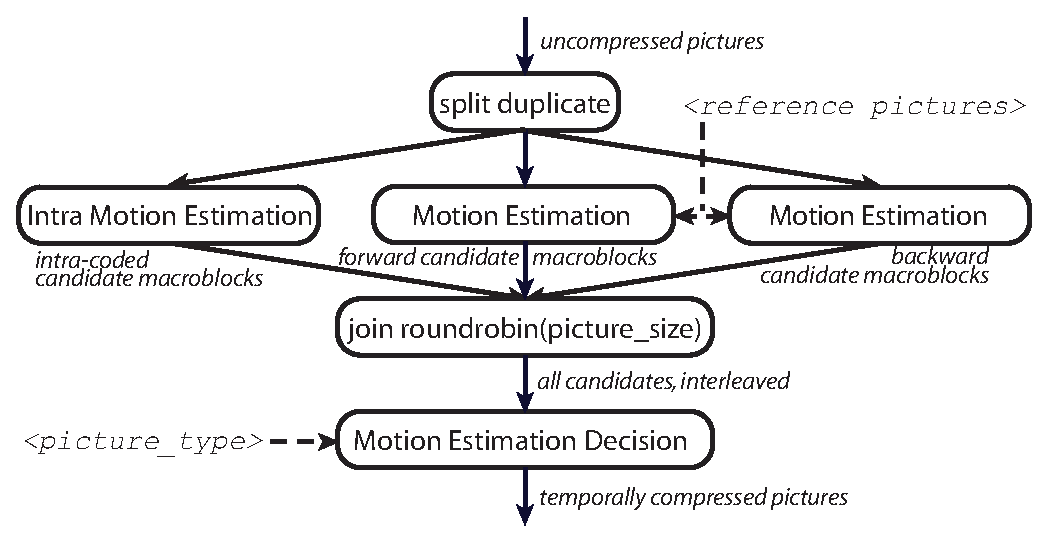
\includegraphics[scale=0.6, angle=0]{./motion_estimation.eps}
    \caption{Motion estimation stream subgraph.}
    \label{fig:motion_estimation_subgraph}
  \end{center}
\end{figure}

Each of the two motion estimation filters receives messages 
containing the previous reference frame to use for estimation. 
The reference frame is the reference 
frame {\em as the decoder would see it} so the actual 
reference pictures are not determined till near the end of the 
overall MPEG-2 pipeline. The MPEG-2 encoder thus relies on 
upstream messages to carry the reference pictures back. 
Upstream messages are defined with respect to the data being 
received by the sender, rather than the data being pushed, 
but otherwise have the same semantics as ordinary 
messages~\cite{thies05ppopp}.

\section{Implementation Statistics}
\label{section:first_decoder_impl}

The MPEG-2 decoder and encoder implementations are fully functional. 
The codecs support progressive streams which conform to the MPEG-2 Main 
Profile (See~\cite{MPEG2}, P.106). Video parameters such as chrominance 
format and video dimensions are currently set in the source code and the 
application must be recompiled if they change. Code organization and 
installation instructions can be found at the StreamIt MPEG-2 
website~\cite{mpeg-streamit-website} and the code is available 
for download~\cite{mpeg-streamit-download}. The decoder 
implementation required approximately 8 weeks given no prior knowledge 
of any of the MPEG-2 specifications. (I had prior experience with JPEG 
and the StreamIt language.) The encoder implementation followed the 
decoder implementation and required a similar length of time. 
Line counts\footnote{Line 
counts were generated using the \texttt{SLOCcount}~\cite{sloccount} tool. 
It strips whitespace and comments.}
 for the decoder, encoder, and common functionality 
between them, are shown in Table~\ref{table:line_counts}. (All code reused between decoder and 
encoder appears in the shared library number, not in the decoder or encoder 
numbers.) The short implementation time and the size of the code base 
indicates in a rough fashion StreamIt's ability to efficiently express 
the MPEG-2 computation.

\begin{figure}[t]
  \begin{center}
    \begin{tabular}{|l|c|}
\hline
 & Line Count \\
\hline
Decoder & 1357 \\
Encoder & 1513 \\
Shared & 925 \\
\hline
    \end{tabular}
  \end{center}
  \caption{StreamIt line counts for decoder-only, encoder-only, and shared library code.}
  \label{table:line_counts}
\end{figure}

\begin{figure}[t]
  \begin{center}
    \begin{tabular}{|l|c|c|c|}
\hline
        & Filters & Pipelines & Splitjoins \\
\hline
Decoder & 6       & 9         & 9 \\
Encoder & 16      & 15        & 18 \\
Shared  & 17      & 10        & 5 \\
\hline
    \end{tabular}
  \end{center}
  \caption{StreamIt declaration counts for decoder-only, encoder-only, and shared library stream components.}
  \label{table:component_counts}
\end{figure}

Table~\ref{table:component_counts} shows the number of static streams in 
the MPEG-2 codecs. By static streams, I mean the number of components 
programmed by myself. At compile-time, due to multiple instantiation and 
component reuse, the decoder and encoder resolve to stream graphs 
containing between 600 and 6000 components. The range is due to some 
parameterization of the parallelism in the stream graph.

